
\documentclass[a4paper,12pt]{article}
%%%%%%%%%%%%%%%%%%%%%%%%%%%%%%%%%%%%%%%%%%%%%%%%%%%%%%%%%%%%%%%%%%%%%%%%%%%%%%%%%%%%%%%%%%%%%%%%%%%%%%%%%%%%%%%%%%%%%%%%%%%%%%%%%%%%%%%%%%%%%%%%%%%%%%%%%%%%%%%%%%%%%%%%%%%%%%%%%%%%%%%%%%%%%%%%%%%%%%%%%%%%%%%%%%%%%%%%%%%%%%%%%%%%%%%%%%%%%%%%%%%%%%%%%%%%
\usepackage{eurosym}
\usepackage{vmargin}
\usepackage{amsmath}
\usepackage{graphics}
\usepackage{epsfig}
\usepackage{framed}
\usepackage{subfigure}
\usepackage{fancyhdr}
\usepackage{framed}
\usepackage{subfiles}
\usepackage{graphics}
\usepackage{newlfont}
\usepackage{eurosym}
\usepackage{amsmath,amsthm,amsfonts}
\usepackage{amsmath}
\usepackage{enumerate}
\usepackage{color}
\usepackage{multicol}
\usepackage{amssymb}
\usepackage{multicol}
\usepackage[dvipsnames]{xcolor}
\usepackage{graphicx}

\setcounter{MaxMatrixCols}{10}
%TCIDATA{OutputFilter=LATEX.DLL}
%TCIDATA{Version=5.00.0.2570}
%TCIDATA{<META NAME="SaveForMode"CONTENT="1">}
%TCIDATA{LastRevised=Wednesday, February 23, 201113:24:34}
%TCIDATA{<META NAME="GraphicsSave" CONTENT="32">}
%TCIDATA{Language=American English}

\pagestyle{fancy}
\setmarginsrb{20mm}{0mm}{20mm}{25mm}{12mm}{11mm}{0mm}{11mm}
\lhead{MA4128} \rhead{Kevin O'Brien} \chead{Binary Classification} %\input{tcilatex}

%http://www.electronics.dit.ie/staff/ysemenova/Opto2/CO_IntroLab.pdf
\begin{document}

\section*{Binary Classification}
\subsection*{What Is Classification}
Classification is the problem of identifying to which of a set of categories
(sub-populations) a new observation belongs, on the basis of a training set
of data containing observations (or instances) whose category membership is
known. 

% Logisticn Rege Discriminant analysis is an example of a classification method.
\begin{itemize}
	\item  To train (create) a classifier, the fitting function estimates the parameters
	of a Gaussian distribution for each class.
	\item  To predict the classes of new data, the trained classifier finds the class
	with the smallest misclassification cost.
\end{itemize}
\subsection*{Types I and II Error}
A type I error is the incorrect rejection of a true null hypothesis. A type
II error is the failure to reject a false null hypothesis. A type I error is a
false positive. Usually a type I error leads one to conclude that a thing or
relationship exists when really it doesn’t. A type II error is a false negative.
\begin{figure}[h!]
	\centering
	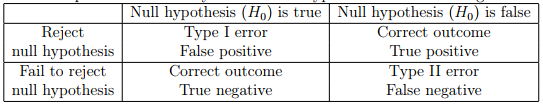
\includegraphics[width=0.7\linewidth]{Table}
	% \caption{}
	% \label{fig:table}
\end{figure}

\subsection*{False Positive and False Negative Error}

\begin{itemize}
	\item 
	A false positive error, commonly called a ``\textbf{false alarm}``, is a result that indicates
	a given condition has been fulfilled, when it actually has not been
	fulfilled. A false positive error is a Type I error % where the test is checking a single condition, and results in an affirmative or negative decision usually
	% designated as ”true or false”.
	\item  A false negative error is where a test result indicates that a condition
	failed, while it actually was successful. A false negative error is a Type II
	error.% occurring in test steps where a single condition is checked for and the 	result can either be positive or negative.
\end{itemize}

\subsection{ROC Curves}
\begin{itemize}
	\item  A receiver operating characteristic (ROC), or ROC curve, is a graphical plot that illustrates
	the performance of a binary classification system as its discrimination threshold is varied.
	\item  The ROC curve is created by plotting the true positive rate against the false positive rate at
	various threshold settings. (The true-positive rate is also known as sensitivity in biomedicine,
	or recall in machine learning. The false-positive rate is also known as the fall-out and can be
	calculated as 1 - specificity).
	\item  The ROC curve was first developed by electrical engineers and radar engineers during World
	War II for detecting enemy objects in battlefields. ROC analysis since then has been used in
	medicine, radiology, biometrics, and other areas for many decades and is increasingly used
	in machine learning and data mining research.
	\item  The ROC is also known as a relative operating characteristic curve, because it is a comparison
	of two operating characteristics (TPR and FPR) as the criterion changes.
\end{itemize}
%====================================================%
\subsection{Properties of ROC Curves}
An ROC curve demonstrates several things:
1. It shows the tradeoff between sensitivity and specificity (any increase in sensitivity will be
accompanied by a decrease in specificity).
2. The closer the curve follows the upper-left border of the ROC space, the more accurate the
test.
3. The closer the curve comes to the 45-degree diagonal of the ROC space, the less accurate the
test.
4. The slope of the tangent line at a cutpoint gives the likelihood ratio (LR) for that value of
the test.
5. The Area Under the Curve is a measure of accuracy.
Figure 1: Receiver Operating Characteristic (ROC) curve

%====================================================%
\begin{itemize}
	\item  In a Receiver Operating Characteristic (ROC) curve the true positive rate (Sensitivity) is
	plotted in function of the false positive rate (100-Specificity) for different cut-off points.
	\item  Each point on the ROC curve represents a sensitivity/specificity pair corresponding to a
	particular decision threshold.
	
	\item  A test with perfect discrimination (no overlap in the two distributions) has a ROC curve that
	passes through the upper left corner (100% sensitivity, 100% specificity).
	\item  Therefore the closer the ROC curve is to the upper left corner, the higher the overall accuracy
	of the test.
	
\end{itemize}
\newpage

In statistics, a receiver operating characteristic (ROC), or ROC curve, is a graphical plot that illustrates the performance of a binary classifier system as its discrimination threshold is varied. The curve is created by plotting the true positive rate against the false positive rate at various threshold settings. (The true-positive rate is also known as sensitivity in biomedicine, or recall in machine learning. The false-positive rate is also known as the fall-out and can be calculated as 1 - specificity). 

The ROC curve is thus the sensitivity as a function of fall-out. In general, if the probability distributions for both detection and false alarm are known, the ROC curve can be generated by plotting the cumulative distribution function (area under the probability distribution from $-\infty$ to $+\infty$) of the detection probability in the y-axis versus the cumulative distribution function of the false-alarm probability in x-axis.
ROC analysis provides tools to select possibly optimal models and to discard suboptimal ones independently from (and prior to specifying) the cost context or the class distribution. ROC analysis is related in a direct and natural way to cost/benefit analysis of diagnostic decision making.
The ROC curve was first developed by electrical engineers and radar engineers during World War II for detecting enemy objects in battlefields and was soon introduced to psychology to account for perceptual detection of stimuli. ROC analysis since then has been used in medicine, radiology, biometrics, and other areas for many decades and is increasingly used in machine learning and data mining research.
The ROC is also known as a relative operating characteristic curve, because it is a comparison of two operating characteristics (TPR and FPR) as the criterion changes.
\subsection*{Receiver Operating Characteristic (ROC) curve}
In a Receiver Operating Characteristic (ROC) curve the true positive rate
(Sensitivity) is plotted in function of the false positive rate (100-Specificity)
for different cut-off points. Each point on the ROC curve represents a sensitivity/specificity
pair corresponding to a particular decision threshold. A
test with perfect discrimination (no overlap in the two distributions) has a
ROC curve that passes through the upper left corner (100% sensitivity, 100%
specificity). Therefore the closer the ROC curve is to the upper left corner,
the higher the overall accuracy of the test (Zweig and Campbell, 1993).

\subsection*{Receiver Operating Characteristic (ROC) curve}
\begin{figure}
	\centering
	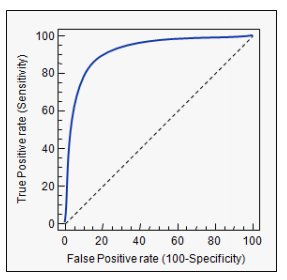
\includegraphics[width=0.55\linewidth]{ROCcurve}
	\caption{}
	\label{fig:roccurve}
\end{figure}
\begin{itemize}
	\item In a Receiver Operating Characteristic (ROC) curve the true positive rate
	(Sensitivity) is plotted in function of the false positive rate (100-Specificity)
	for different cut-off points. 
	\item Each point on the ROC curve represents a sensitivity/specificity
	pair corresponding to a particular decision threshold. 
	\item A
	test with perfect discrimination (no overlap in the two distributions) has a
	ROC curve that passes through the upper left corner (100\% sensitivity, 100\%
	specificity). 
	\item Therefore the closer the ROC curve is to the upper left corner,
	the higher the overall accuracy of the test. %(Zweig and Campbell, 1993).
\end{itemize}



\end{document}